\documentclass[a4paper,ngerman]{article}

\usepackage[ngerman]{babel}
\usepackage[utf8]{inputenc}
\usepackage[
    pdftitle={DiVe - Distance Vector Routing Simulation},
	pdfsubject={Eine kurze Beschreibung, worum es geht},
	pdfauthor={Nico Kratky},
	pdfkeywords={meta, information, pdf, hyperref, latex}
]{hyperref}
\usepackage{fancyvrb}
\usepackage{minted}
\usepackage{graphicx}
\usepackage[section]{placeins}

\graphicspath{{images/}}

\title{%
    DiVe \\
    Distance Vector Routing Simulation
}
\author{Nico Kratky}

\begin{document}

\begin{titlepage}
\maketitle
\end{titlepage}

\tableofcontents
\clearpage

\section{Lizenz}
\begin{Verbatim}[fontsize=\small]
Boost Software License - Version 1.0 - August 17th, 2003

Permission is hereby granted, free of charge, to any person or organization
obtaining a copy of the software and accompanying documentation covered by
this license (the "Software") to use, reproduce, display, distribute,
execute, and transmit the Software, and to prepare derivative works of the
Software, and to permit third-parties to whom the Software is furnished to
do so, all subject to the following:

The copyright notices in the Software and this entire statement, including
the above license grant, this restriction and the following disclaimer,
must be included in all copies of the Software, in whole or in part, and
all derivative works of the Software, unless such copies or derivative
works are solely in the form of machine-executable object code generated by
a source language processor.

THE SOFTWARE IS PROVIDED "AS IS", WITHOUT WARRANTY OF ANY KIND, EXPRESS OR
IMPLIED, INCLUDING BUT NOT LIMITED TO THE WARRANTIES OF MERCHANTABILITY,
FITNESS FOR A PARTICULAR PURPOSE, TITLE AND NON-INFRINGEMENT. IN NO EVENT
SHALL THE COPYRIGHT HOLDERS OR ANYONE DISTRIBUTING THE SOFTWARE BE LIABLE
FOR ANY DAMAGES OR OTHER LIABILITY, WHETHER IN CONTRACT, TORT OR OTHERWISE,
ARISING FROM, OUT OF OR IN CONNECTION WITH THE SOFTWARE OR THE USE OR OTHER
DEALINGS IN THE SOFTWARE.

My apologies. When the previous paragraph was written, lowercase had not yet
been invented (that would involve another several millennia of evolution).
I did not mean to shout.
\end{Verbatim}
\clearpage

\section{Aufgabenstellung}

Die Aufgabe besteht darin ein C++-Programm zur Simulation des Distanzvektor-Algorithmus zu entwickeln. Zusätzlich zum Algorithmus sollen zufällige Ausfälle der Verbindungen simuliert werden können.

\subsection{Verwendete Technologien}

Die zu verwendenden Technologien wurden vorgegeben. Nur Google Protocol Buffers wurden zusätzlich verwendet.

\begin{itemize}
    \item C++14
    \item CMake und make
    \item \{fmt\}
    \item spdlog
    \item JSON for Modern C++
    \item Asio (standalone Variante)
    \item Google Protocol Buffers
\end{itemize}

\subsection{Distanzvektor-Algorithmus}

Der Distanzvektor-Algorithmus ist eines der einfacheren Routing Protokolle. Es handelt nach dem Prinzip "Teile deinen Nachbarn mit, wie du die Welt siehst".

\section{Konzeption}

Für die Implementation der Simulation wurde nur ein einziges Programm entwickelt. Die Netzwerktopologie kann durch mehrmaliges starten auf entweder verschiedenen Rechnern oder auf ein und demselben Rechner aufgebaut werden. Diese Topologie wird in einer JSON Konfigurationsdatei festgelegt.

\subsection{Klassenstruktur}

% insert UML Diagram

\subsection{Programmablauf}

\section{Konfiguration der Topologie}

Die Netzwerktopologie kann durch eine JSON Konfigurationsdatei festgelegt werden. Eine Beispielkonfigurationsdatei ist im Appendix \ref{appendix:config} zu finden. Diese definiert eine Netzwerktopologie wie sie Abbildung \ref{fig:topology} zeigt.

\begin{figure}[H]
    \centering
    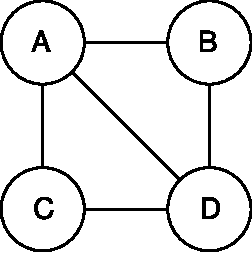
\includegraphics[width=4cm,keepaspectratio]{topology2}
    \caption{Dies ist eine Caption}
    \label{fig:topology}
\end{figure}

Die Reihenfolge zwischen den Link Elementen macht hierbei nur einen Unterschied falls ein \textit{pof} Wert gesetzt ist. \textit{pof} steht hierbei für \textit{probability of failure}, was soviel bedeutet wie Ausfallwahrscheinlichkeit. Dieser Wert muss zwischen 0 und 1 liegen und gibt diese Wahrscheinlichkeit des Ausfalls der Verbindung von \textit{source} nach \textit{target} in Prozent an. Der Unterschied ist jedoch nicht für den Nutzer sichtbar. Er besteht lediglich in der Implementierung, da nur der \textit{source} Knoten berechnet ob ein Ausfall vorliegt und falls dies der Fall ist es an den \textit{target} Knoten weitergibt.

\section{Kommandozeile}

Als Benutzerschnittstelle werden Kommandozeilenparameter verwendet. Es gibt zwei Parameter die zwingend übergeben werden müssen. Dies sind einerseits die JSON Konfigurationsdatei und andererseits die Router ID. Die Router ID bestimmt welchen Router der eben gestartete Prozess in der konfigurierten Topologie widerspiegelt. Das Interval in dem die Routing Updates gesendet werden, kann durch den \textit{-i} bzw. \textit{--interval} eingestellt werden. Hier muss ein ganzzahliger Wert übergeben werden. Voreingestellt sind 5 Sekunden. Wenn der \textit{-v} bzw. \textit{--verbose} Parameter übergeben wird, dann werden zusätzliche Information ausgegeben.

\begin{Verbatim}
SYNOPSIS
        ./router <topology file> <router id> [-i <seconds>] [-v]

OPTIONS
        -i, --interval
                    router update interval (default: 5)

        -v, --verbose
                    print additional debug information
\end{Verbatim}

\section{Netzwerkübertragung}

\clearpage
\begin{appendix}

\section{Beispielkonfigurationsdatei}
\label{appendix:config}

\begin{minted}{json}
{
    "nodes": {
        "A": {
            "ip_address": "127.0.0.1",
            "port": 16022
        },
        "B": {
            "ip_address": "127.0.0.1",
            "port": 16023
        },
        "C": {
            "ip_address": "127.0.0.1",
            "port": 16024
        },
        "D": {
            "ip_address": "127.0.0.1",
            "port": 16025
        }
    },
    "links": [
        {
            "source": "A",
            "target": "D"
        },
        {
            "source": "A",
            "target": "B"
        },
        {
            "source": "A",
            "target": "C"
        },
        {
            "source": "B",
            "target": "D"
        },
        {
            "source": "C",
            "target": "D"
        }
        ]
}
\end{minted}

\end{appendix}

\end{document}
